\documentclass[a4paper, 10pt, twoside]{article}
\usepackage[left=2cm, right=2cm, top=2cm, bottom=3cm]{geometry}
\usepackage{amsmath}
\usepackage[shortlabels]{enumitem}
\usepackage{bbold}
\usepackage{cases}
\usepackage{systeme}
\usepackage{graphicx}

\begin{document}



\title{Algorithm Theory - Assignment 1}
\author{T\'eo Bouvard}
\maketitle

\section*{Problem 1}
In this problem, the objective is to maximize the profit of selling products X and Y, while satisfying production constraints on these products. The profit can be computed as

\begin{align*}
    profit & = revenue - cost                                                                              \\
           & = revenue - (time_{machine} \times cost_{machine} + time_{craftsman} \times cost_{craftsman})
\end{align*}

We can compute profits for each of the products

\begin{align*}
    profit(X) = 200 - (\frac{15}{60} \times 100 + \frac{20}{60} \times 20) = \frac{505}{3} \\
    profit(Y) = 300 - (\frac{20}{60} \times 100 + \frac{30}{60} \times 20) = \frac{770}{3}
\end{align*}

And formulate the problem as a Linear Programming problem. Let $n_X$ and $n_Y$ be the number of products X and Y produced.

\begin{align*}
     & \text{maximize } n_X \times profit(X) + n_Y \times profit(Y) \\
     & \text{subject to }
    \begin{cases}
        n_X \times time_{machine}(X) + n_Y \times time_{machine}(Y) \le 40 \times 60     \\
        n_X \times time_{craftsman}(X) + n_Y \times time_{craftsman}(Y) \le 35 \times 60 \\
        n_X \ge 10                                                                       \\
        n_X, n_Y \ge 0                                                                   \\
    \end{cases}
\end{align*}

Which can be simplified as

\begin{align*}
     & \text{maximize } n_X \times \frac{505}{3} + n_Y \times \frac{770}{3} \\
     & \text{subject to }
    \begin{cases}
        15 \times n_X + 20 \times n_Y \le 2400 \\
        20 \times n_X + 30 \times n_Y \le 2100 \\
        n_X \ge 10                             \\
        n_Y \ge 0                              \\
    \end{cases}
\end{align*}

\section*{Problem 2}
\begin{enumerate}[a)]
    \item

          Let $n_{A}$ and $n_{B}$ be the number of products A and B produced.

          \begin{align*}
               & \text{maximize } n_{A} \times 3 + n_{B} \times 5 \\
               & \text{subject to }
              \begin{cases}
                  12 \times n_{A} + 25 \times n_{B} \le 30 \times 60 \\
                  2 \times n_{B} - 5 \times n_{A} \ge 0              \\
                  n_{A}, n_{B} \ge 0                                 \\
              \end{cases}
          \end{align*}

          \begin{center}
              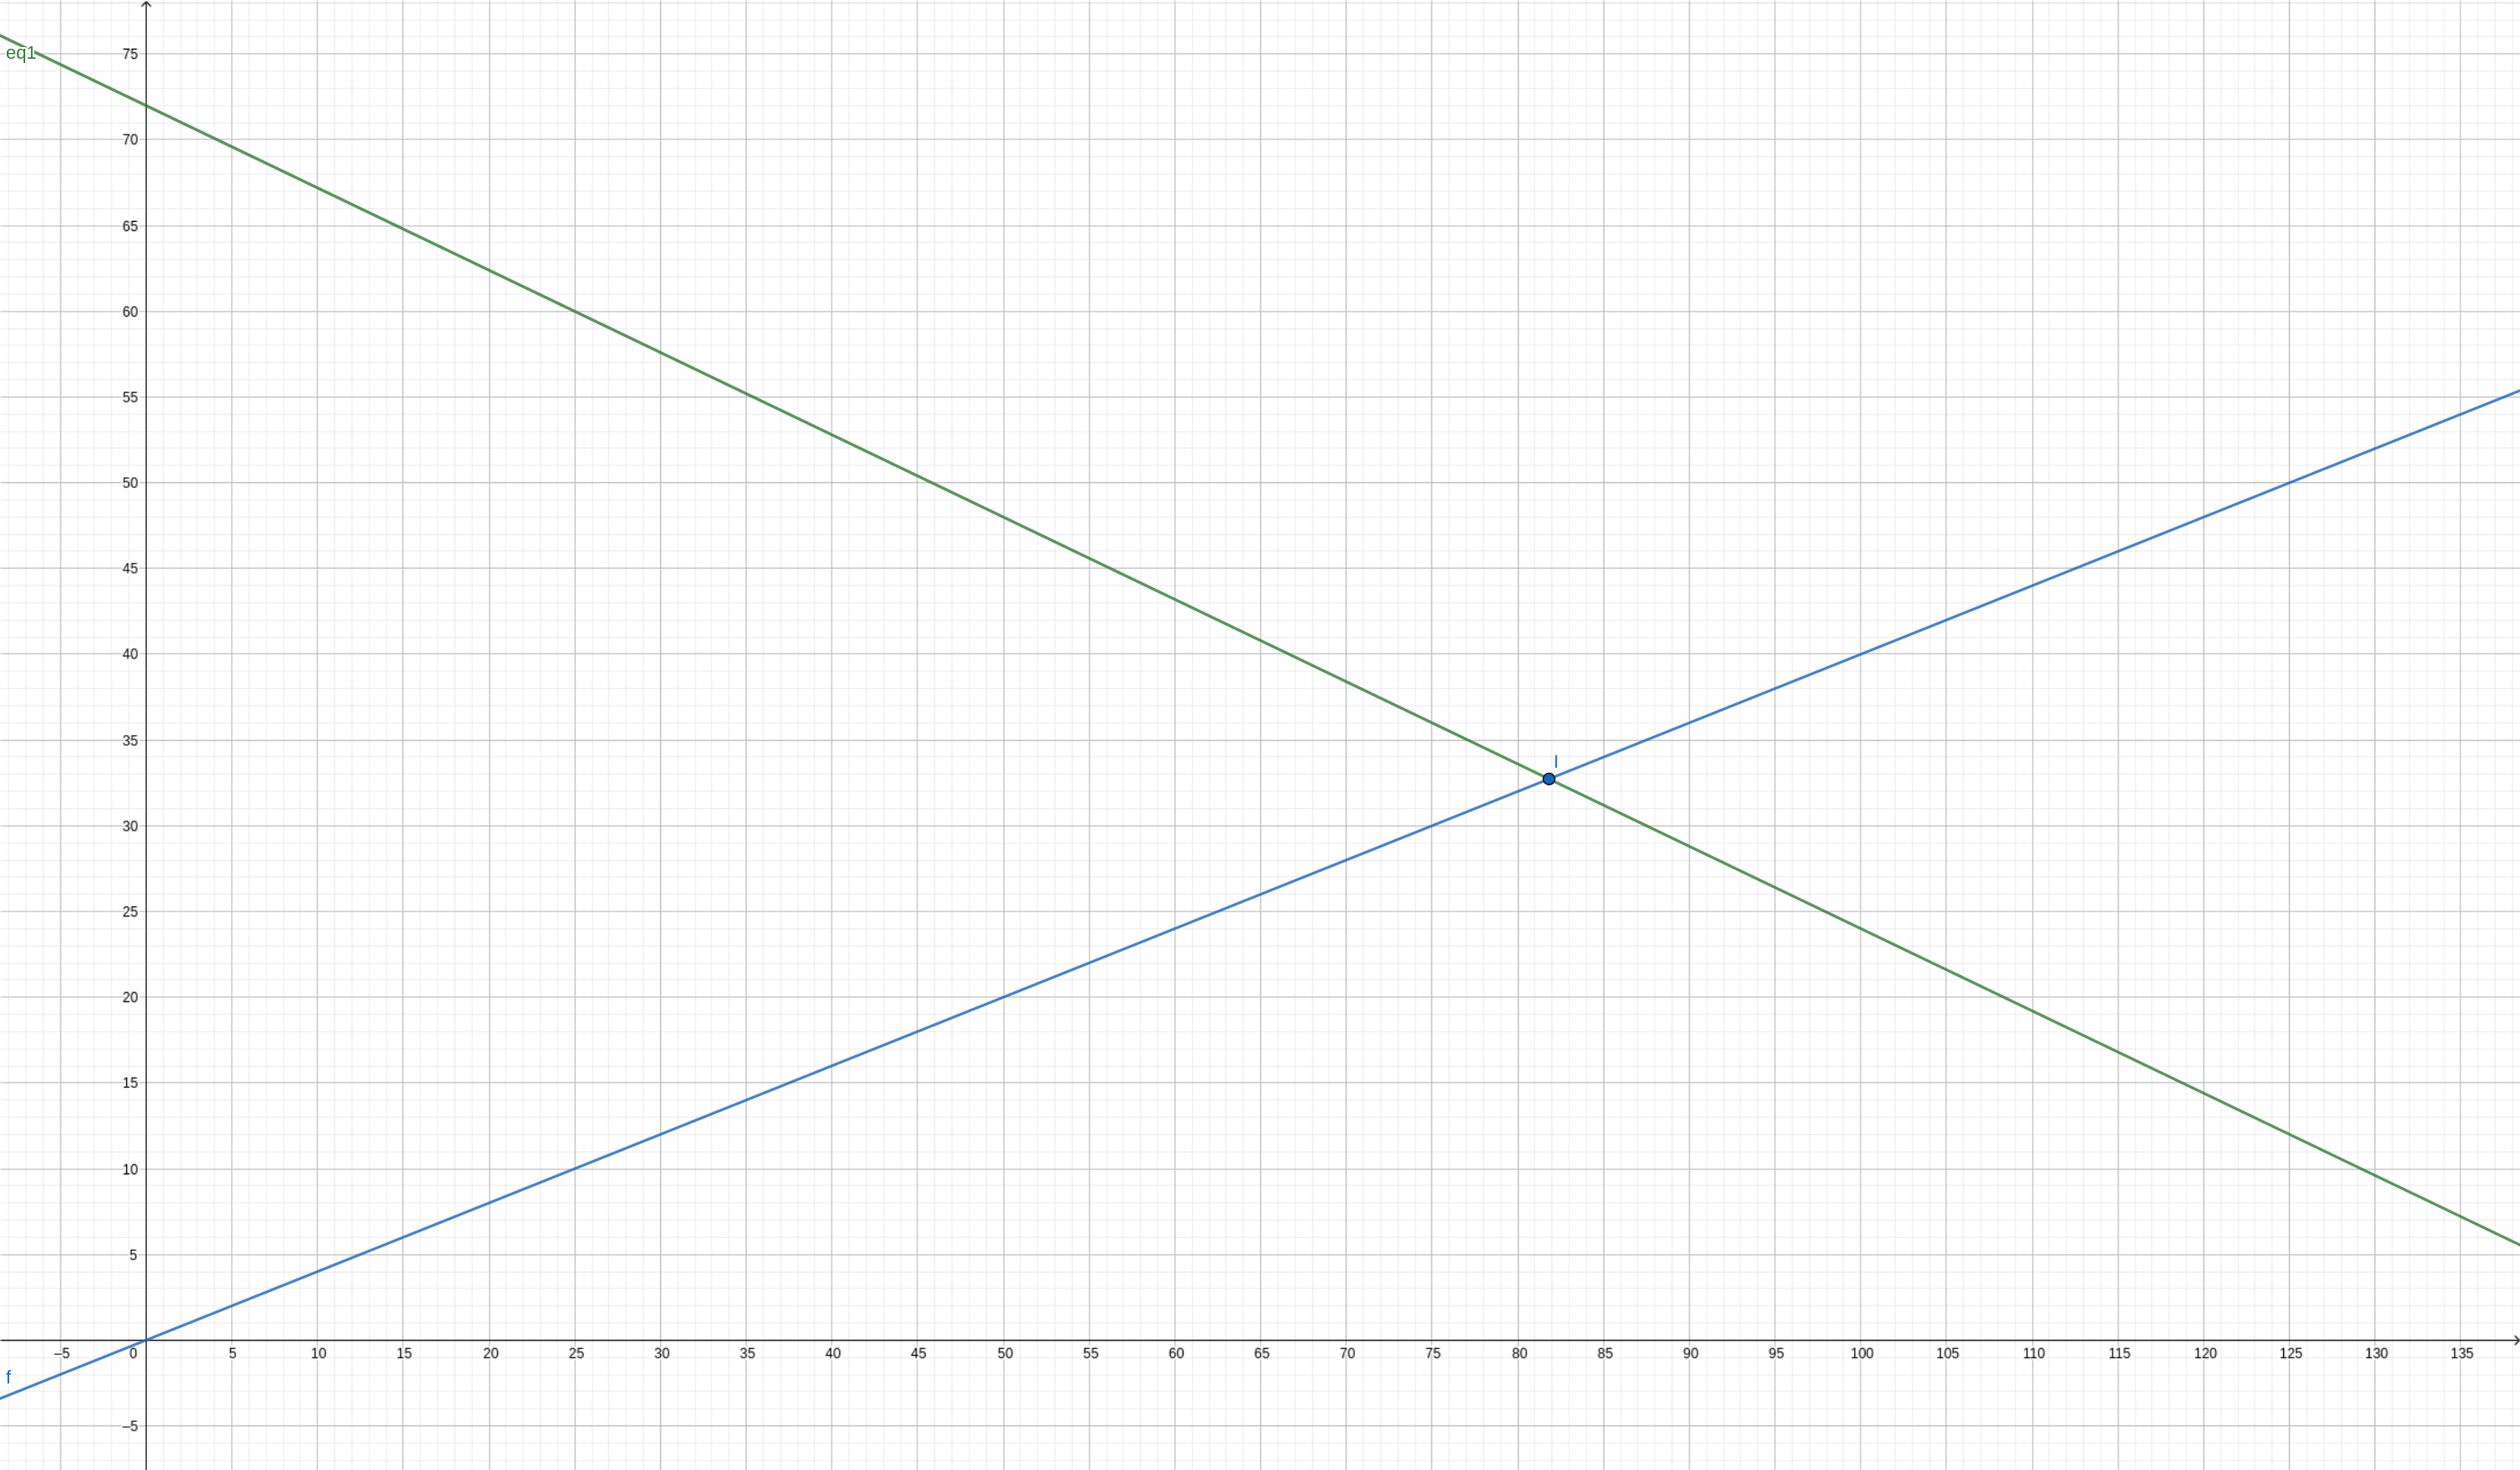
\includegraphics[width = .5 \textwidth]{graph.png}
          \end{center}

          By graphing the feasible region, we see three candidate points. The first one $I_0 = (0, 0)$ can be trivially discarded as it leads to a profit of 0\$. Let's evaluate the objective function at the two other points. At $I_1 = (72, 0)$ the profit is 216\$. To compute the coordinates of the last point, we solve the following system.

          %\begin{align*}
          %    \systeme{
          %        12 \times n_{A} + 25 \times n_{B} = 1800,
          %        2 \times n_{B} - 5 \times n_{A} = 0
          %    }
          %    \implies
          %    \systeme{
          %        22 \times n_{A} = 1800,
          %        n_{B} = \frac{2}{5} \times n_{A}
          %    }
          %    \implies
          %    \systeme{
          %        n_{A} = 81.8,
          %        n_{B} = 32.7
          %    }
          %\end{align*}

          and at $I_2 = (81.8, 32.7)$ the profit is 408.9\$ which is the highest profit in this case. However, $n_A$ and $n_B$ are not integers. It is not specified in the exercise whether they should be or not, but as the problem is about a weekly production, we can assume that they do not need to be integer quantities as the weeks are continuous. If we wanted to optimal integer solution, we should pick $n_A = 81$ and $n_B = 33$, leading to a profit of 408\$.

        \item By doubling the production capacity without modifying the other constraints, the resulting profit is doubled. The company should then pay less than 408\$ for renting an extra machine thath is profitable.
\end{enumerate}

\section*{Problem 3}

\begin{enumerate}[a)]
    \item We want to minimize the total cost of transportation, while respecting constraints on the flights. This problem can be formulated as the following linear programming problem.
    Let $n_{A}$ and $n_{B}$ be the number of flights flown with aircrafts A and B respectively. 

    \begin{align*}
        & \text{minimize } n_{A} \times 10000 + n_{B} \times 12000 \\
        & \text{subject to }
       \begin{cases}
           30 \times n_{A} + 15 \times n_{B} \ge 300 \\
           500 \times n_{A} - 750 \times n_{B} \ge 9000 \\
           n_{A} + n_{B} \le 16 \\
           n_{A}, n_{B} \ge 0 \\
       \end{cases}
   \end{align*}

   With the graph method, we can identify the three points delimiting the feasible region. We first determine their coordinates, and then evaluate the objective function at these points.

    \begin{align*}
        I_1 : 
        \systeme{
            30x+15y=300,
            x+y=16
        }
        \implies
        \systeme[.]{
            x=4,
            y=12
        }
        \implies \text{cost } = 184000\,\$ \\
        I_2 : 
        \systeme{
            30x+15y=300,
            500x+750y=9000
        }
        \implies
        \systeme[.]{
            x=6,
            y=8
        }
        \implies \text{cost } = 156000\,\$ \\
        I_3 : 
        \systeme{
            x+y=16,
            500x+750y=9000
        }
        \implies
        \systeme[.]{
            x=12,
            y=4
        }
        \implies \text{cost } = 168000\,\$ \\
    \end{align*}

    The lowest cost is achieved by using 6 flights with A and 8 flights with B, for a total cost of 156000\$.
   
\end{enumerate}

\section*{Problem 4}

\begin{enumerate}[a)]
    \item Graph method
    
    \begin{align*}
        I_2 : 
        \systeme[]{
            x_1 = 0,
            x_2 = 0
        }
        \implies \text{objective } = 0 \\
        I_3 : 
        \systeme[]{
            x_1 = 30,
            x_2 = 0
        }
        \implies \text{objective } = 90 \\
        I_3 : 
        \systeme[]{
            x_1 = 0,
            x_2 = 25
        }
        \implies \text{objective } = 125 \\
        I_1 : 
        \systeme{
            x_1+2x_2=50,
            8x_1+3x_2=240
        }
        \implies
        \systeme[]{
            x_1 = \frac{490}{13},
            x_2 = \frac{160}{13}
        }
        \implies \text{objective } = \frac{2270}{13} \approx 174.6 \\
    \end{align*}

    \item Simplex algorithm

    We first convert the linear problem its the slack form by introducing two variables $s_1$ and $s_2$.

    \begin{align*}
        &\text{maximize } z = 3x_1 + 5x_2 \\
        &\text{subject to }
        \begin{cases}
            x_1 + 2x_2 + s_1 = 50 \\
            8x_1 + 3x_2 + s_2 = 240 \\
            x_1, x_2, s_1, s_2 \ge 0 \\
        \end{cases}    
    \end{align*}

    A basic feasible solution is $(x_1, x_2, s_1, s_2) = (0, 0, 50, 240)$. We choose $x_2$ as the entering variable as it has the highest coefficient in the objective function. To choose the leaving variable, we find the tightest constraint on $x_2$. In the first constraint, $x_2$ is limited to 25, and in the second constraint it is limited to 80. Thus the leaving variable is $s_1$ We rewrite the problem by switching the entering and the leaving variable. $x_2 = 25 - \frac{x_1}{2} - \frac{s_1}{2}$

    \begin{align*}
        &\text{maximize } z = 125 + \frac{x_1}{2} - \frac{5}{2}s_1 \\
        &\text{subject to }
        \begin{cases}
            50-x_1-2x_2 = s_1 \\
            8x_1 + 3x_2 + s_2 = 240 \\
            x_1, x_2, s_1, s_2 \ge 0 \\
        \end{cases}    
    \end{align*}

    The only remaining entering variable able to increase the objective function is $x_1$. 
\end{enumerate}


\end{document}
